\documentclass[aspectratio=169]{beamer}
\usepackage[utf8]{inputenc}
\usepackage[T1]{fontenc}
\usepackage{lmodern}
\usepackage[english]{babel}
\usepackage{graphicx}
\usepackage{caption}
\usepackage{subfigure}
\usepackage[export]{adjustbox}
\usepackage{multirow}
\usepackage{booktabs}
\usepackage{colortbl}
\usepackage{xcolor}
\usepackage{hyperref}
\usetheme{Boadilla}
%\usetheme{default}


\usepackage[backend=bibtex]{biblatex}
\addbibresource{references}


\newcommand\blfootnote[1]{%
  \begingroup
  \renewcommand\thefootnote{}\footnote{#1}%
  \addtocounter{footnote}{-1}%
  \endgroup
}

\captionsetup{font=scriptsize,labelfont=scriptsize}

\AtBeginSection[]
{
    \begin{frame}
        \frametitle{Outline}
        \tableofcontents[currentsection]
    \end{frame}
}

\setbeamertemplate{footline}[frame number]
\setbeamertemplate{navigation symbols}{}
\setbeamertemplate{items}[square]
\setbeamertemplate{section in toc}[square]
%\setbeamertemplate{itemize items}[default]
%\setbeamertemplate{enumerate items}[default]

\setbeamertemplate{itemize/enumerate body begin}{\normalsize}
\setbeamertemplate{itemize/enumerate subbody begin}{\normalsize}

\definecolor{light-gray}{gray}{0.9}


\title[COMPSTAT 2024]{Univariate Time Series Forecasting using Echo State Networks: An Empirical Application}
\subtitle{26th International Conference on Computational Statistics}
\author[Alexander Häußer]{Alexander Häußer \blfootnote{\tiny{\url{alexander.haeusser@wirtschaft.uni-giessen.de}}}}
\institute[]{Justus-Liebig-University Giessen \\ Faculty 02 - Economics and Business Studies \\ Chair of Statistics and Econometrics}
\date{August 27, 2024}



\begin{document}

\begin{frame}
\titlepage
\end{frame}

\begin{frame}
\frametitle{Outline}
\tableofcontents
\end{frame}


\section{Introduction}

\begin{frame}[t]{Introduction}
    \begin{minipage}[t]{0.5\textwidth}
        \vspace{0pt}
        \textbf{Research objectives}
        \begin{itemize}
        	\item Develop an algorithm for fast and fully automatic time series modeling and forecasting using Echo State Networks (ESN)
        	\item Benchmark approach against state-of-the-art forecasting methods
        	\item Functions available in the R package \href{https://github.com/ahaeusser/echos}{\texttt{echos}}
        \end{itemize}
    \end{minipage}%
    \hfill
    \begin{minipage}[t]{0.5\textwidth}
        \vspace{0pt}
        \textbf{Experimental setup}
        \begin{itemize}
        	\item Data from the M4 Forecasting Competition
        		\begin{itemize}
        			\item 2,400 monthly and 1,200 quarterly time series
        			\item Forecast horizon $h = 18$ for monthly and $h = 8$ for quarterly data
        		\end{itemize}
        	\item Evaluate forecast accuracy (MASE, sMAPE) and measure computational run-time
        	\item Compare against simple methods, statistical models and neural networks
        \end{itemize}
    \end{minipage}
\end{frame}



\section{Echo State Networks}



\begin{frame}[t]{Echo State Network - Architecture}
    \begin{minipage}[t]{0.3\textwidth}
        \vspace{0pt}
        \begin{itemize}
			\item Input $u_{t} = y_{t-1}$ is non-linearly expanded into a high-dimensional feature space (i.e., internal states)
			\item Output $y_{t}$ is combined via trainable weights from these internal states
			\item Dashed lines indicate fixed weights ($\boldsymbol{\omega}^{in}$, $\boldsymbol{\omega}$) and solid lines indicate trainable weights $\boldsymbol{\omega}^{out}$
        \end{itemize}
    \end{minipage}%
    \hfill
    \begin{minipage}[t]{0.7\textwidth}
        \vspace{0pt}
 		\begin{figure}[H]
		\center
			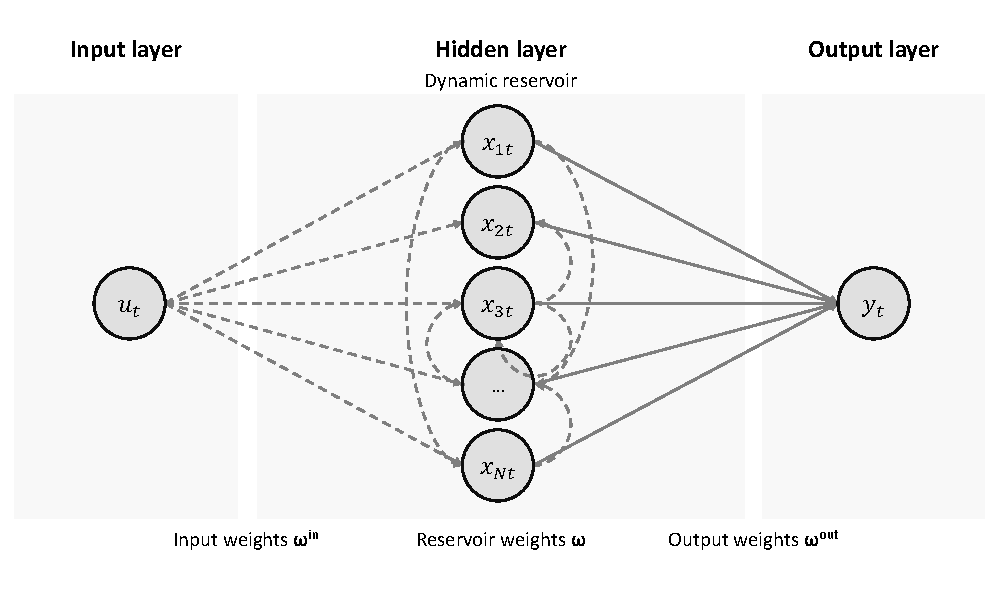
\includegraphics[scale=0.6]{figures/figure_04_architecture.pdf}
		\end{figure}
    \end{minipage}
\end{frame}







\begin{frame}[t]{Echo State Network - Basic model\footnote{More details in the appendix}}
    \begin{minipage}[t]{0.33\textwidth}
        \vspace{0pt}
        \textbf{1. Data pre-processing}
        \begin{itemize}
            \item Identify non-stationarity via KPSS test
			\item If required, calculate (first) difference to remove non-stationarity
			\item Scale (stationary) time series to interval $[-0.5, 0.5]$
        \end{itemize}
    \end{minipage}%
    \hfill
    \begin{minipage}[t]{0.33\textwidth}
        \vspace{0pt}
        \textbf{2. Reservoir generation}
        \begin{itemize}
            \item Calculate the internal states according to
				\begin{equation*}
					\mathbf{x}_{t} = \tanh \left( {\boldsymbol{\omega}^{in}} u_{t} + \boldsymbol{\omega} \mathbf{x}_{t-1} \right)
				\end{equation*}
			\item First autoregressive lag as input, i.e., $u(t) = y(t-1)$
			\item Input and reservoir weight matrices $\boldsymbol{\omega}^{in}$ and $\boldsymbol{\omega}$
			\item Collect internal states in design matrix $\mathbf{X} = [\mathbf{1},  x_{1t}, x_{2t}, ..., x_{Nt}]$
        \end{itemize}
    \end{minipage}
    \hfill
    \begin{minipage}[t]{0.33\textwidth}
        \vspace{0pt}
        \textbf{3. Model estimation and selection}
        \begin{itemize}
            \item Linear model
            	\begin{equation*}
            	\mathbf{y} = \mathbf{X} \boldsymbol{\omega}^{out} + \boldsymbol{\epsilon}
				\end{equation*}
			\item Estimate coefficients via ridge regression
				\begin{equation*}
				\boldsymbol{\hat{\omega}}^{out} = (\mathbf{X}^\top \mathbf{X} + \mathbf{R}_{\lambda})^{-1}\mathbf{X}^\top\mathbf{y}
				\end{equation*}
			\item Regularization parameter $\lambda$ is determined via random search by minimizing the BIC
        \end{itemize}
    \end{minipage}
\end{frame}




\begin{frame}[t]{Data from the M4 Forecasting Competition}
    \begin{minipage}[t]{0.3\textwidth}
        \vspace{0pt}
        \begin{itemize}
            \item Original M4 dataset consists of 100,000 time series
			\item Different frequencies and applications fields
			\item Randomly selected 2,400 monthly and 1,200 quarterly series
			\item Diverse dataset with different characteristics (trend, season, non-stationarity, etc.)
        \end{itemize}
    \end{minipage}%
    \hfill
    \begin{minipage}[t]{0.7\textwidth}
        \vspace{0pt}
 		\begin{figure}[H]
		\center
			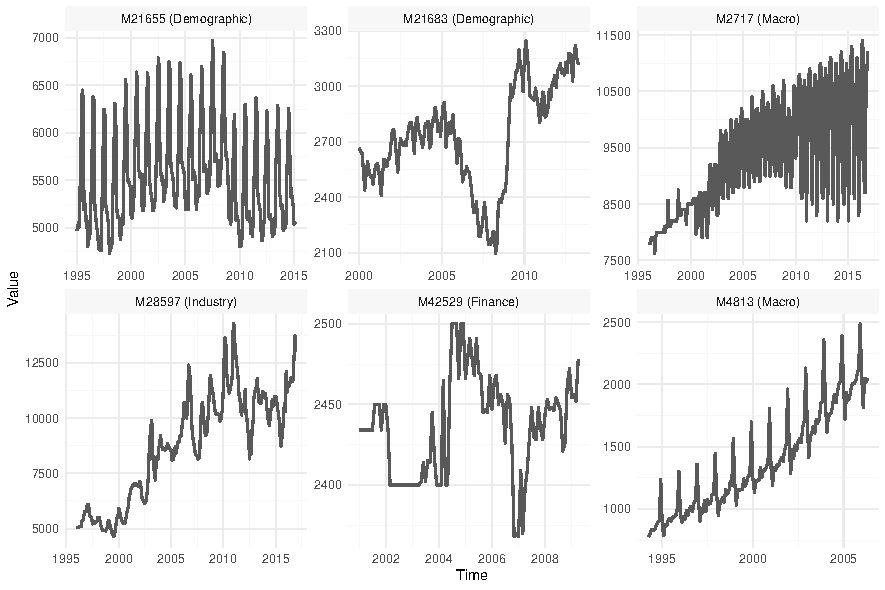
\includegraphics[scale=0.7]{figures/figure_03_data_sample_wide.pdf}
		\end{figure}
    \end{minipage}
\end{frame}



\begin{frame}[t]{Reservoir generation - Feature engineering using the echo state approach}
    \begin{minipage}[t]{0.3\textwidth}
        \vspace{0pt}
        \begin{itemize}
            \item Internal states (colored lines) and the pre-processed output variable (black line)
			\item Non-linear dimensionality expansion as a feature engineering technique for time series
			\item Problems
				\begin{itemize}
					\item Multicollinearity
					\item Overfitting
					\item ...
				\end{itemize}
        \end{itemize}
    \end{minipage}%
    \hfill
    \begin{minipage}[t]{0.7\textwidth}
        \vspace{0pt}
 		\begin{figure}[H]
		\center
			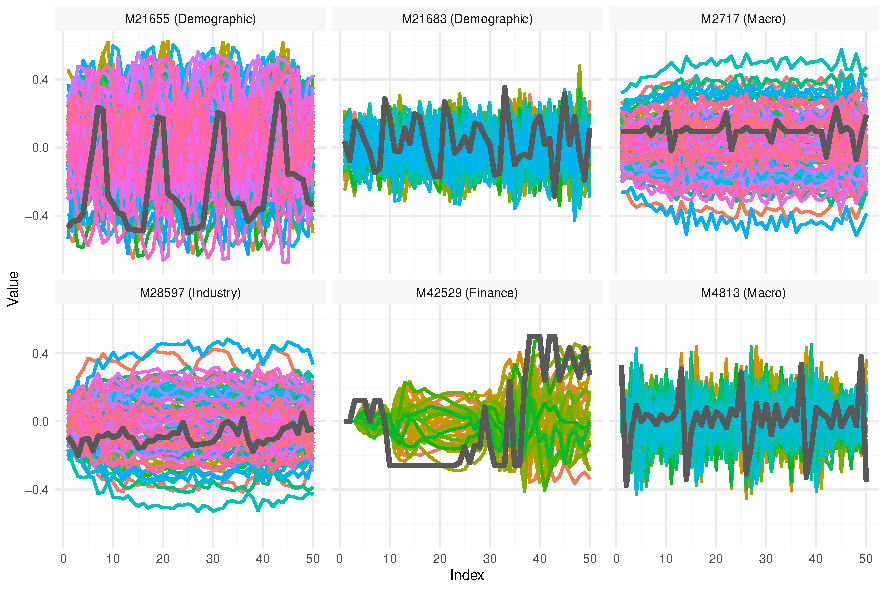
\includegraphics[scale=0.7]{figures/figure_05_model_states_wide.pdf}
		\end{figure}
    \end{minipage}
\end{frame}



\begin{frame}[t]{Model selection and estimation - Random search and ridge regression}
    \begin{minipage}[t]{0.3\textwidth}
        \vspace{0pt}
        \begin{itemize}
            \item Top 5 internal states (colored lines) and the pre-processed output variable (black line)
			\item Selection based on the size of the absolute value of the coefficients (high correlation $\rightarrow$ predictive power)
			\item Lead-lag relationship captures auto-correlation, seasonality, etc.
        \end{itemize}
    \end{minipage}%
    \hfill
    \begin{minipage}[t]{0.7\textwidth}
        \vspace{0pt}
 		\begin{figure}[H]
		\center
			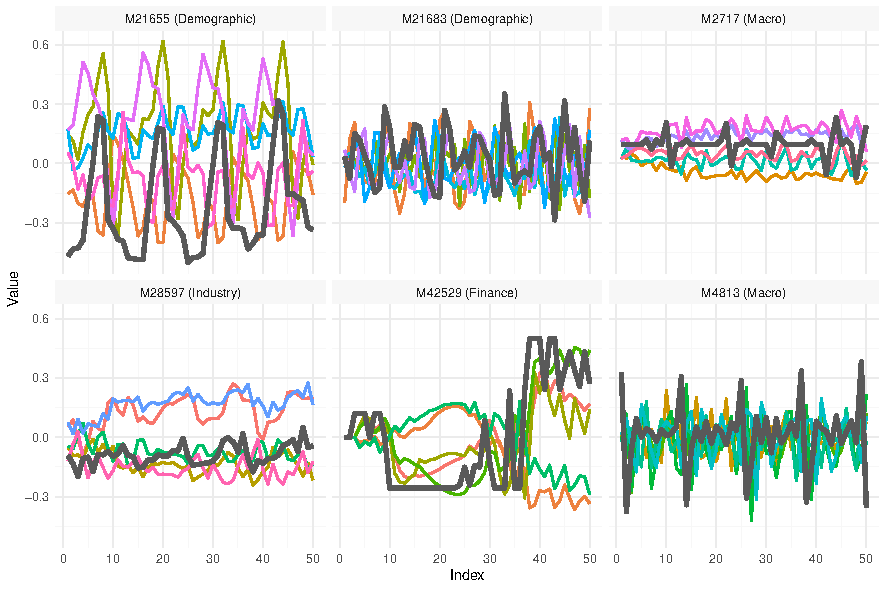
\includegraphics[scale=0.7]{figures/figure_06_model_states_top_wide.pdf}
		\end{figure}
    \end{minipage}
\end{frame}


\begin{frame}[t]{Actual values, fitted values and forecasts from trained ESN}
    \begin{minipage}[t]{0.3\textwidth}
        \vspace{0pt}
        \begin{itemize}
        	\item Recursive forecasting due to \textit{autoregressive nature}
            \item Actual values (black), fitted values (red) and out-of-sample forecasts (green)
			\item Vertical dotted line: split into training and testing (holdout)
			\item ESN model produces reasonable forecasts
        \end{itemize}
    \end{minipage}%
    \hfill
    \begin{minipage}[t]{0.7\textwidth}
        \vspace{0pt}
 		\begin{figure}[H]
		\center
			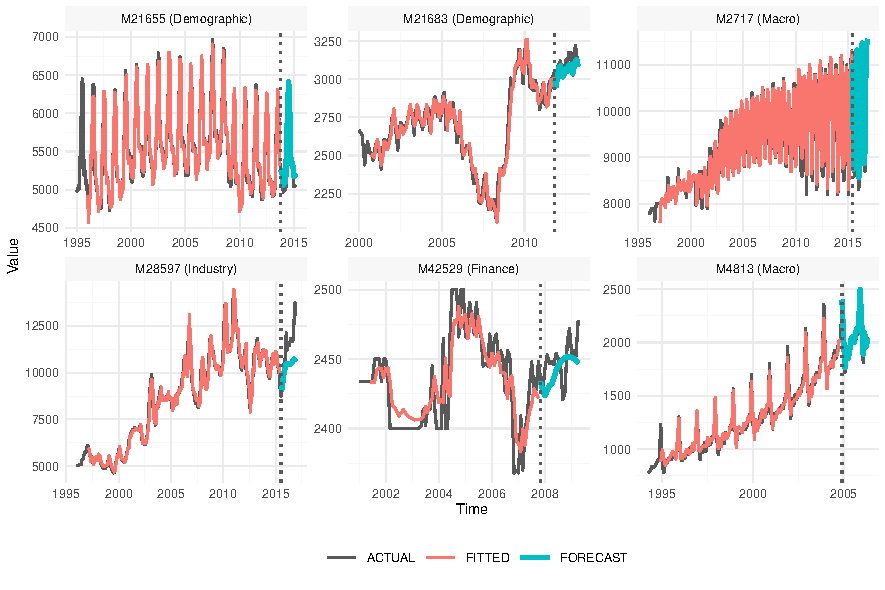
\includegraphics[scale=0.7]{figures/figure_07_model_forecast_sample_wide.pdf}
		\end{figure}
    \end{minipage}
\end{frame}



\section{Empirical application}

\begin{frame}[t]{Monthly dataset - Forecast accuracy and run-time}
    \begin{minipage}[t]{0.3\textwidth}
        \vspace{0pt}
        \textbf{Key takeaways}
        \begin{itemize}                      
            \item ESN achieved very good results in terms of forecast accuracy and run-time
            \item Differences between the top methods are marginal
			\item Statistical methods outperform neural networks
        \end{itemize}
    \end{minipage}%
    \hfill
    \begin{minipage}[t]{0.7\textwidth}
        \vspace{0pt}
 		\begin{table}[ht]
			\scriptsize
			\centering
			\begin{tabular}{lrrrrrr}
				\toprule
				\multirow{2}{*}{\textbf{Model}} & \multicolumn{2}{c}{\textbf{MASE}} & \multicolumn{2}{c} {\textbf{sMAPE [\%]}} & \multicolumn{2}{c}{\textbf{Run Time [sec]}} \\
				\cmidrule(l){2-3} \cmidrule(l){4-5} \cmidrule(l){6-7}
 				& Mean & Median & Mean  & Median & Mean & Total \\
				\midrule
				\rowcolor{light-gray} ESN & \textbf{0.885} & 0.717 & 17.877 & 12.296 & 0.201 & 483.406 \\ 
				TBATS & 0.887 & \textbf{0.711} & 17.075 & 12.246 & 0.650 & 1561.136 \\ 
				ARIMA & 0.891 & 0.729 & 17.963 & 12.415 & 0.256 & 613.874 \\ 
				ETS & 0.902 & 0.722 & 17.763 & \textbf{12.182} & 0.167 & 401.617 \\ 
				THETA & 0.902 & 0.716 & \textbf{16.814} & 12.196 & 0.024 & 58.558 \\ 
				ELM & 0.930 & 0.739 & 18.430 & 13.081 & 23.995 & 57588.779 \\ 
				MLP & 1.026 & 0.839 & 21.398 & 14.637 & 2.209 & 5302.472 \\ 
				NNETAR & 1.042 & 0.830 & 19.663 & 14.374 & 39.318 & 94363.406 \\ 
				DRIFT & 1.077 & 0.806 & 20.013 & 13.750 & 0.025 & 60.752 \\ 
				NAIVE & 1.097 & 0.847 & 19.573 & 14.419 & 0.030 & 72.308 \\ 
				PROPHET & 1.143 & 0.890 & 23.901 & 15.859 & 0.783 & 1879.991 \\ 
				SNAIVE & 1.165 & 0.948 & 20.489 & 15.770 & 0.025 & 60.429 \\ 
				TSLM & 1.538 & 1.156 & 31.740 & 20.203 & 0.030 & 71.990 \\ 
				MEDIAN & 2.841 & 1.788 & 37.020 & 31.912 & \textbf{0.024} & \textbf{56.925} \\ 
				MEAN & 2.849 & 1.958 & 38.178 & 33.766 & 0.026 & 61.436 \\ 
				\bottomrule
			\end{tabular}
		\end{table}
    \end{minipage}
\end{frame}




\begin{frame}[t]{Quarterly dataset - Forecast accuracy and run-time}
    \begin{minipage}[t]{0.3\textwidth}
        \vspace{0pt}
        \textbf{Key takeaways}
        \begin{itemize}
			\item ESN achieved good results in terms of forecast accuracy and run-time
			\item Statistical methods outperform neural networks
        \end{itemize}
    \end{minipage}%
    \hfill
    \begin{minipage}[t]{0.7\textwidth}
        \vspace{0pt}
 		\begin{table}[ht]
			\scriptsize
			\centering
			\begin{tabular}{lrrrrrr}
				\toprule
				\multirow{2}{*}{\textbf{Model}} & \multicolumn{2}{c}{\textbf{MASE}} & \multicolumn{2}{c}					{\textbf{sMAPE [\%]}} & \multicolumn{2}{c}{\textbf{Run Time [sec]}} \\
				\cmidrule(l){2-3} \cmidrule(l){4-5} \cmidrule(l){6-7}
 				& Mean & Median & Mean  & Median & Mean & Total \\
				\midrule
				ETS & \textbf{1.082} & \textbf{0.839} & 10.264 & 5.398 & 0.062 & 74.100 \\ 
				TBATS & 1.104 & 0.843 & \textbf{9.975} & 5.579 & 0.336 & 403.254 \\ 
				ELM & 1.114 & 0.880 & 10.771 & \textbf{5.352} & 1.382 & 1658.841 \\ 
				\rowcolor{light-gray} ESN & 1.114 & 0.908 & 10.672 & 5.540 & 0.052 & 61.836 \\ 
				ARIMA & 1.119 & 0.876 & 10.410 & 5.703 & 0.106 & 127.593 \\ 
				THETA & 1.150 & 0.908 & 10.339 & 5.859 & 0.026 & 31.040 \\ 
				DRIFT & 1.155 & 0.888 & 10.915 & 5.524 & 0.025 & 30.375 \\ 
				MLP & 1.187 & 0.917 & 11.673 & 5.833 & 0.602 & 722.079 \\ 
				NAIVE & 1.329 & 1.070 & 11.358 & 6.813 & 0.035 & 41.978 \\ 
				PROPHET & 1.435 & 1.089 & 14.316 & 7.070 & 1.653 & 1983.211 \\ 
				NNETAR & 1.444 & 1.126 & 12.793 & 7.358 & 25.078 & 30093.072 \\ 
				SNAIVE & 1.513 & 1.282 & 12.753 & 8.003 & 0.025 & 29.628 \\ 
				TSLM & 1.879 & 1.478 & 16.222 & 9.759 & 0.028 & 33.849 \\ 
				MEAN & 4.241 & 3.567 & 29.691 & 24.863 & \textbf{0.024} & \textbf{28.402} \\ 
				MEDIAN & 4.361 & 3.510 & 31.259 & 24.729 & 0.024 & 29.179 \\ 
				\bottomrule
			\end{tabular}
		\end{table}
    \end{minipage}
\end{frame}



\section{Summary}


\begin{frame}[t]{Summary and outlook}
    \begin{minipage}[t]{0.5\textwidth}
        \vspace{0pt}
        \textbf{Summary}
        \begin{itemize}
            \item Proposed model achieved high accuracy and can outperform or compete against state-of-the-art forecasting methods
            \item Empirical results demonstrate the universal learning capabilities and the potential of ESNs
            \begin{itemize}
            	\item Data-driven instead of model-driven forecasts
            	\item Being more generic and making less assumptions
            \end{itemize}
        \end{itemize}
    \end{minipage}%
    \hfill
    \begin{minipage}[t]{0.5\textwidth}
        \vspace{0pt}
        \textbf{Outlook}
        \begin{itemize}
        	\item Probabilistic forecasting, i.e., enhance point forecasts with forecast distributions
        	\item Multivariate forecasting and exogenous inputs
        	\item Reservoir generation as feature engineering technique
        \end{itemize}
    \end{minipage}
\end{frame}


\section{References}

\begin{frame}[allowframebreaks]
    \frametitle{References}
    \nocite{*}
    \printbibliography[heading=none]
\end{frame}


\section{Appendix}

\begin{frame}[t]{Echo State Network  - Settings and hyperparameters (1/2)}
    \begin{minipage}[t]{0.3\textwidth}
        \vspace{0pt}
        \textbf{Reservoir generation}
        \begin{itemize}
        	\item Input weight matrix $\boldsymbol{\omega}^{in} \in \mathbb{R}^{N \times 1}$ and the reservoir weight matrix $\boldsymbol{\omega} \in \mathbb{R}^{N \times N}$ are generated randomly
        	\item Dynamic rules for determining the number of internal states, initial drop-out, etc.
        \end{itemize}
    \end{minipage}%
    \hfill
    \begin{minipage}[t]{0.7\textwidth}
        \vspace{0pt}
        	\begin{table}[ht]
        	\scriptsize
			\centering
				\begin{tabular}{ll}
				\toprule
				\textbf{Setting}                                    & \textbf{Value/Formula}               \\
				\midrule
				Input ($\mathbf{u}$)                                & $y_{t-1}$                            \\
				Output ($\mathbf{y}$)                               & $y_{t}$                              \\
				Activation function                                 & $tanh(.)$                            \\
				Internal states                                     & $N = min(\lfloor 0.4T \rfloor, 100)$ \\
				Initial drop-out                                    & $\delta = \lfloor 0.05T \rfloor$     \\
				\midrule
				Input weight matrix ($\boldsymbol{\omega}^{in}$)    &                                      \\
				\hspace{2.5mm} Dimension                            & $N \times 1$                         \\
				\hspace{2.5mm} Random uniform                       & $[-0.5, 0.5]$                        \\
				\hspace{2.5mm} Density                              & 100\%                                \\
				\midrule
				Reservoir weight matrix ($\boldsymbol{\omega}$)     &                                      \\
				\hspace{2.5mm} Dimension                            & $N \times N$                         \\
				\hspace{2.5mm} Random uniform                       & $[-0.5, 0.5]$                        \\
				\hspace{2.5mm} Density                              & 50\%                                 \\
				\hspace{2.5mm} Spectral radius                      & $\rho = 1.0$                         \\
				\bottomrule
				\end{tabular}
			\end{table}
    \end{minipage}
\end{frame}



\begin{frame}[t]{Echo State Network  - Settings and hyperparameters (2/2)}
    \begin{minipage}[t]{0.3\textwidth}
        \vspace{0pt}
        \textbf{Model estimation and selection}
        \begin{itemize}
        	\item Ridge Regression reduces overfitting and eliminates difficulties with ill-posed optimization problems
        	\item Regularization parameter $\lambda$ optimized via random search
        	\item Effective degrees of freedom to determine model complexity in BIC
        \end{itemize}
    \end{minipage}%
    \hfill
    \begin{minipage}[t]{0.7\textwidth}
        \vspace{0pt}
        	\begin{table}[ht]
        	\scriptsize
			\centering
				\begin{tabular}{ll}
				\toprule
				\textbf{Setting}                          & \textbf{Value/Formula}	 \\
				\midrule
				Model type                                & $\mathbf{y} = \mathbf{X} \boldsymbol{\omega}^{out} + \boldsymbol{\epsilon}$	 \\
				Output weight matrix                      & $\boldsymbol{\hat{\omega}}^{out} = (\mathbf{X}^\top \mathbf{X} + \mathbf{R}_{\lambda})^{-1}\mathbf{X}^\top\mathbf{y}$ \\
				Optimization algorithm                    & Random search 	 \\
				Search space ($\lambda$)                  &  				 \\
				\hspace{2.5mm} Number of random values    & $K = 2N$             \\
				\hspace{2.5mm} Interval of random uniform & $[10^{-4}, 2]$   \\
				Information criterion                     & $BIC_{\lambda} = -2 L + \ln(T) df_{\lambda}$ \\
				Effective degrees of freedom	          & $df_{\lambda} = tr[{\mathbf{X}{{({\mathbf{X}^{\top}\mathbf{X} + \mathbf{R}_{\lambda}})}^{ - 1}}\mathbf{X}^{\top}}]$ \\
				\bottomrule
				\end{tabular}
			\end{table}
    \end{minipage}
\end{frame}


\begin{frame}[t]{Monthly dataset - Number of obs. and strength of trend and seasonality}
	\begin{figure}[H]
    \center
		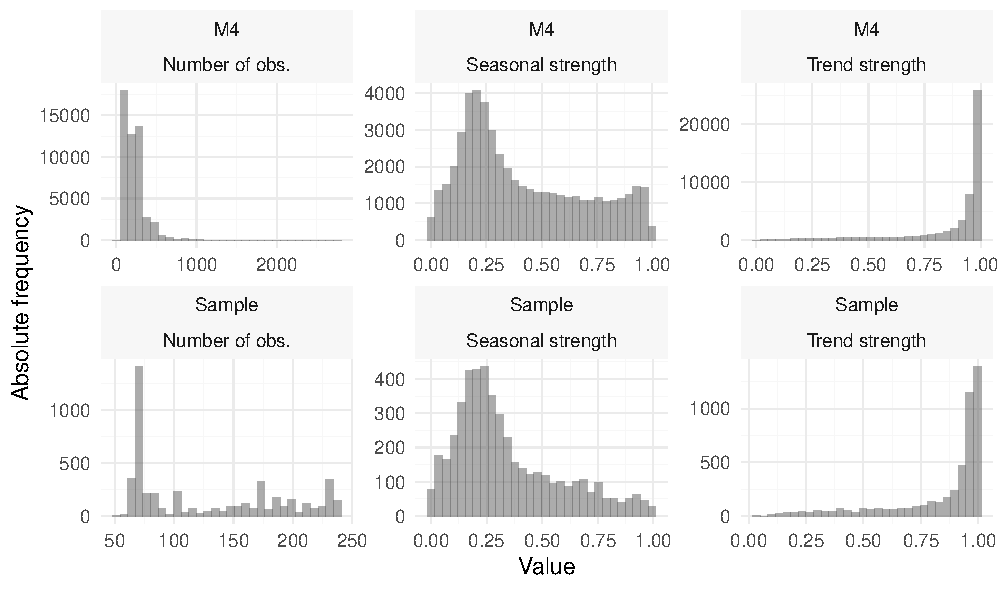
\includegraphics[scale=0.7]{figures/figure_01_data_monthly.pdf}
	\end{figure}
\end{frame}


\begin{frame}[t]{Quarterly dataset - Number of obs. and strength of trend and seasonality}
	\begin{figure}[H]
    \center
		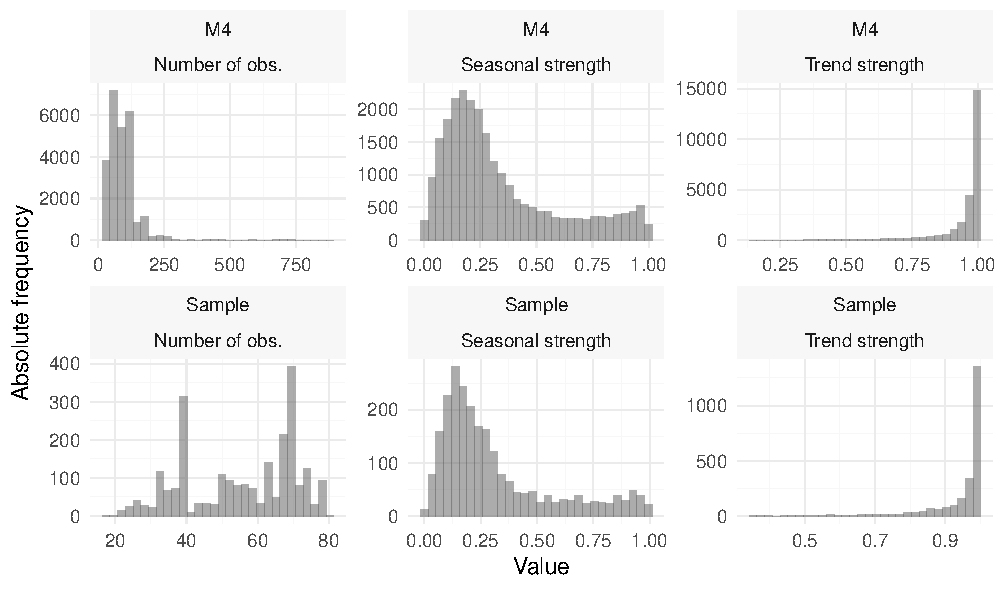
\includegraphics[scale=0.7]{figures/figure_02_data_quarterly.pdf}
	\end{figure}
\end{frame}


\end{document}
